\documentclass[12pt,a4paper]{article}
% ── Paquetes ───────────────────────────────────────────────────────────────────
\usepackage[utf8]{inputenc}
\usepackage[spanish]{babel}
\usepackage{amsmath}
\usepackage{graphicx}
\usepackage{listings}
\usepackage{xcolor}
\usepackage{hyperref}
\usepackage{geometry}
\usepackage{enumitem}
\usepackage{fancyhdr}
\usepackage{caption}
\geometry{margin=2.5cm}
% ── Estilo de código ──────────────────────────────────────────────────────────
\lstset{
    language=Python,
    basicstyle=\ttfamily\small,
    keywordstyle=\color{blue},
    stringstyle=\color{red},
    commentstyle=\color{green!50!black},
    numbers=left,
    numberstyle=\tiny,
    frame=single,
    breaklines=true,
    backgroundcolor=\color{gray!5},
}
% ── Configuración de página ───────────────────────────────────────────────────
\pagestyle{fancy}
\fancyhf{}
\fancyhead[L]{\textbf{MeteoApp} -- Manual de Usuario}
\fancyhead[R]{\thepage}
\setlength{\headheight}{14pt}
% ── Título ─────────────────────────────────────────────────────────────────────
\title{\Huge \textbf{MeteoApp}\\[0.3cm]
       \Large Dashboard Meteorológico Personal\\[0.3cm]
       \large Manual de Usuario}
\author{Valentina Rodriguez Sepulveda\\[0.2cm]
        \small ID: 1125789977\\[0.2cm]
        \small Programación II\\[0.2cm]
        \small Universidad Tecnológica de Pereira}
\date{2026}
\begin{document}
\maketitle
\thispagestyle{empty}
\newpage
\tableofcontents
\newpage
% ===============================================================================
\section{Información del Proyecto}
% ===============================================================================
\begin{tabular}{|l|l|}
\hline
\textbf{Título} & MeteoApp -- Dashboard Meteorológico Personal \\
\hline
\textbf{Autor} & Valentina Rodriguez Sepulveda \\
\hline
\textbf{ID} & 1125789977 \\
\hline
\textbf{Asignatura} & Programación II\\
\hline
\textbf{Fecha de entrega} & 2026 \\
\hline
\end{tabular}
% ===============================================================================
\section{Descripción de la Aplicación}
% ===============================================================================
MeteoApp es una aplicación de escritorio desarrollada en Python que funciona como una \textbf{estación meteorológica digital}. Se conecta a internet para consultar datos climáticos reales de cualquier ciudad del mundo a través de la API pública gratuita de \textbf{Open-Meteo} y los presenta al usuario mediante una interfaz gráfica intuitiva construida con \textbf{Flet}.
\subsection{Objetivo}
Proveer al usuario una herramienta visual y fácil de usar para consultar el clima actual, visualizar tendencias históricas y configurar alertas personalizadas de temperatura, todo desde una misma aplicación de escritorio.
\subsection{Funcionalidad general}
\begin{itemize}[itemsep=4pt]
    \item \textbf{Inicio de sesión y registro} de usuarios con contraseñas protegidas mediante hash SHA-256.
    \item \textbf{Consulta del clima actual} de cualquier ciudad del mundo: temperatura, sensación térmica, humedad, viento e ícono del clima.
    \item \textbf{Búsqueda inteligente de ciudades} con geocodificación y selección entre múltiples resultados.
    \item \textbf{Gestión de ciudades favoritas} para acceso rápido.
    \item \textbf{Visualización del historial meteorológico} con gráficas de temperatura (líneas) y precipitación (barras).
    \item \textbf{Configuración de alertas de temperatura} con umbrales máximo y mínimo configurables.
    \item \textbf{Cambio de unidades} entre °C/°F y km/h/mph en tiempo real.
    \item \textbf{Modo offline} con caché local para funcionar sin conexión a internet.
\end{itemize}
% ===============================================================================
\section{Librerías Utilizadas y Almacenamiento}
% ===============================================================================
\subsection{Librerías}
\begin{tabular}{|l|l|l|}
\hline
\textbf{Librería} & \textbf{Versión} & \textbf{Propósito} \\
\hline
Flet & 0.28.3 & Framework de interfaz gráfica (basado en Flutter) \\
Pandas & -- & Manejo de datos tabulares y archivos CSV \\
Requests & -- & Consultas HTTP a la API de Open-Meteo \\
Matplotlib & -- & Generación de gráficas de temperatura y precipitación \\
Pillow & -- & Creación dinámica de íconos del clima \\
\hline
\end{tabular}
\subsection{Tipo de almacenamiento}
La aplicación utiliza \textbf{archivos CSV} (Comma-Separated Values) gestionados con la librería Pandas para la persistencia de datos. Se emplean cuatro archivos:
\begin{itemize}
    \item \textbf{usuarios.csv}: cuentas de usuario (ID, username, password hash, fecha de registro).
    \item \textbf{ciudades.csv}: ciudades favoritas por usuario, coordenadas, umbrales de alerta y último clima consultado.
    \item \textbf{historial\_clima.csv}: datos históricos descargados (caché para evitar consultas repetidas).
    \item \textbf{cache\_clima.csv}: último clima consultado de cada ciudad para modo offline.
\end{itemize}
Los datos se almacenan de forma permanente: al agregar nueva información, los datos existentes no se eliminan. El historial se purga automáticamente después de 365 días para mantener el archivo liviano.
% ===============================================================================
\section{Estructura del Proyecto}
% ===============================================================================
\subsection{Organización de carpetas}

\begin{lstlisting}[frame=none, numbers=none, basicstyle=\ttfamily\footnotesize]
interfaz_grafica_flet/
|-- main.py
|-- requirements.txt
|
|-- utils/
|   |-- api_client.py
|   |-- data_manager.py
|   |-- settings.py
|   \-- chart_generator.py
|
|-- views/
|   |-- login_view.py
|   |-- home_view.py
|   |-- history_view.py
|   |-- cities_view.py
|   \-- alerts_view.py
|
|-- data/
|   |-- usuarios.csv
|   |-- ciudades.csv
|   |-- historial_clima.csv
|   \-- cache_clima.csv
|
\-- assets/
    |-- charts/
    |-- icons/
    \-- screenshots/
\end{lstlisting}

\vspace{0.3cm}
\noindent\textbf{Descripción de cada componente:}

\begin{itemize}[itemsep=3pt]
    \item \textbf{main.py:} punto de entrada de la aplicación y controlador de navegación entre ventanas. Define funciones (\texttt{mostrar\_inicio}, \texttt{mostrar\_historial}, etc.) que limpian la pantalla actual e instancian la vista correspondiente.
    \item \textbf{requirements.txt:} lista de dependencias del proyecto (Flet, Pandas, Requests, Matplotlib, Pillow).
    \item \textbf{utils/api\_client.py:} se comunica con los tres endpoints de la API de Open-Meteo (geocodificación, pronóstico y archivo histórico). Traduce las claves JSON del inglés al español.
    \item \textbf{utils/data\_manager.py:} maneja la lectura y escritura de los cuatro archivos CSV usando Pandas. Contiene las funciones CRUD para usuarios, ciudades, historial y caché.
    \item \textbf{utils/settings.py:} almacena las preferencias globales de unidades (°C/°F, km/h/mph) en variables de módulo para que persistan al navegar entre ventanas.
    \item \textbf{utils/chart\_generator.py:} genera las gráficas PNG (temperatura y precipitación) con Matplotlib usando el backend sin GUI \texttt{Agg}.
    \item \textbf{views/login\_view.py:} pantalla de inicio de sesión y registro. Contiene el \texttt{RadioGroup} con los radio buttons para alternar entre ambos modos.
    \item \textbf{views/home\_view.py:} pantalla principal con el buscador de ciudades, la tarjeta del clima, los botones de unidades y los banners de alerta y modo offline.
    \item \textbf{views/history\_view.py:} pantalla de historial con selector de ciudad (dropdown), selector de fecha (DatePicker), slider de días y dos gráficas generadas con Matplotlib.
    \item \textbf{views/cities\_view.py:} pantalla de gestión de ciudades favoritas con campo de texto para agregar, checkboxes para seleccionar y botón para eliminar las seleccionadas.
    \item \textbf{views/alerts\_view.py:} pantalla de configuración de alertas con dropdown de ciudad, sliders para umbrales de temperatura y checkbox para activar/desactivar la alerta.
    \item \textbf{data/:} carpeta que contiene los cuatro archivos CSV de persistencia. Se crean automáticamente si no existen.
    \item \textbf{assets/charts/:} almacena las gráficas PNG generadas por \texttt{chart\_generator.py} (ej. \texttt{temperatura\_bogotá.png}).
    \item \textbf{assets/icons/:} carpeta reservada para futuros íconos estáticos. Actualmente los íconos del clima se generan dinámicamente en memoria con Pillow (función \texttt{\_crear\_icono()} en \texttt{home\_view.py}) y se codifican en base64, sin necesidad de archivos en disco.
    \item \textbf{assets/screenshots/:} carpeta para las capturas de pantalla de la interfaz utilizadas en este manual.
\end{itemize}
\subsection{Arquitectura de clases}
Cada ventana de la interfaz es una \textbf{clase independiente} con sus propios atributos y métodos, siguiendo el paradigma de Programación Orientada a Objetos (POO):
\begin{itemize}
    \item \texttt{LoginView}: formulario de inicio de sesión y registro con radio buttons para alternar entre modos.
    \item \texttt{HomeView}: pantalla principal con buscador, tarjeta del clima, botones de unidades y banners de alerta.
    \item \texttt{HistoryView}: selector de ciudad y fechas, generación de gráficas y estadísticas del período.
    \item \texttt{CitiesView}: lista de ciudades favoritas con checkboxes para selección múltiple y eliminación.
    \item \texttt{AlertsView}: sliders para configurar umbrales de temperatura y resumen de alertas activas.
\end{itemize}
El archivo \texttt{main.py} actúa como \textbf{controlador de navegación}: limpia la pantalla actual, instancia la nueva vista y la agrega a la página.
% ===============================================================================
\section{Funcionamiento Paso a Paso}
% ===============================================================================
A continuación se describe el funcionamiento de la aplicación con capturas de pantalla de cada pantalla.
\subsection{Inicio de sesión}
Al ejecutar la aplicación, se muestra la pantalla de inicio de sesión. El usuario puede elegir entre "Iniciar sesión" y "Registrarse" mediante radio buttons.
\textbf{Para iniciar sesión:}
\begin{enumerate}
    \item Ingresar nombre de usuario.
    \item Ingresar contraseña.
    \item Hacer clic en "Ingresar".
\end{enumerate}
\textbf{Para registrarse:}
\begin{enumerate}
    \item Seleccionar "Registrarse" con el radio button.
    \item Ingresar usuario y contraseña (mínimo 4 caracteres).
    \item Hacer clic en "Crear cuenta".
\end{enumerate}
Las contraseñas se almacenan como hash SHA-256, nunca en texto plano.
% Imagen: pantalla de login
\begin{figure}[h]
    \centering
    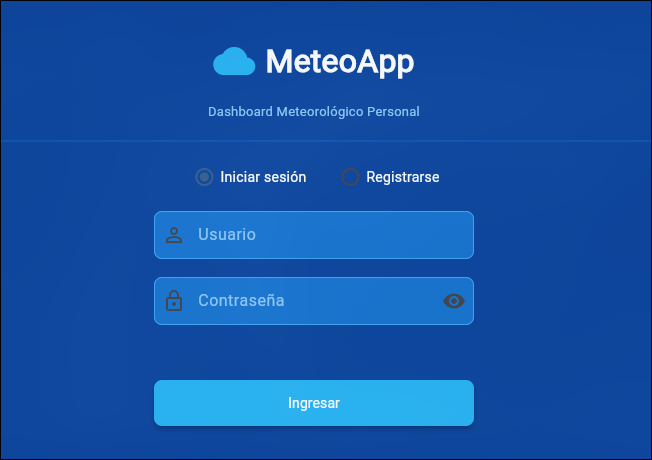
\includegraphics[width=0.7\textwidth]{assets/screenshots/login.png}
    \caption{Pantalla de inicio de sesión con radio buttons para alternar entre login y registro.}
\end{figure}
\subsection{Consulta del clima actual}
Una vez autenticado, se muestra la pantalla principal. Para consultar el clima:
\begin{enumerate}
    \item Escribir el nombre de una ciudad en el campo de búsqueda.
    \item Presionar Enter o hacer clic en "Buscar".
    \item Si hay múltiples resultados, aparece un diálogo para seleccionar la ciudad deseada.
    \item La aplicación muestra una tarjeta con: temperatura, máxima, mínima, sensación térmica, humedad, viento e ícono del clima.
\end{enumerate}
\begin{figure}[h]
    \centering
    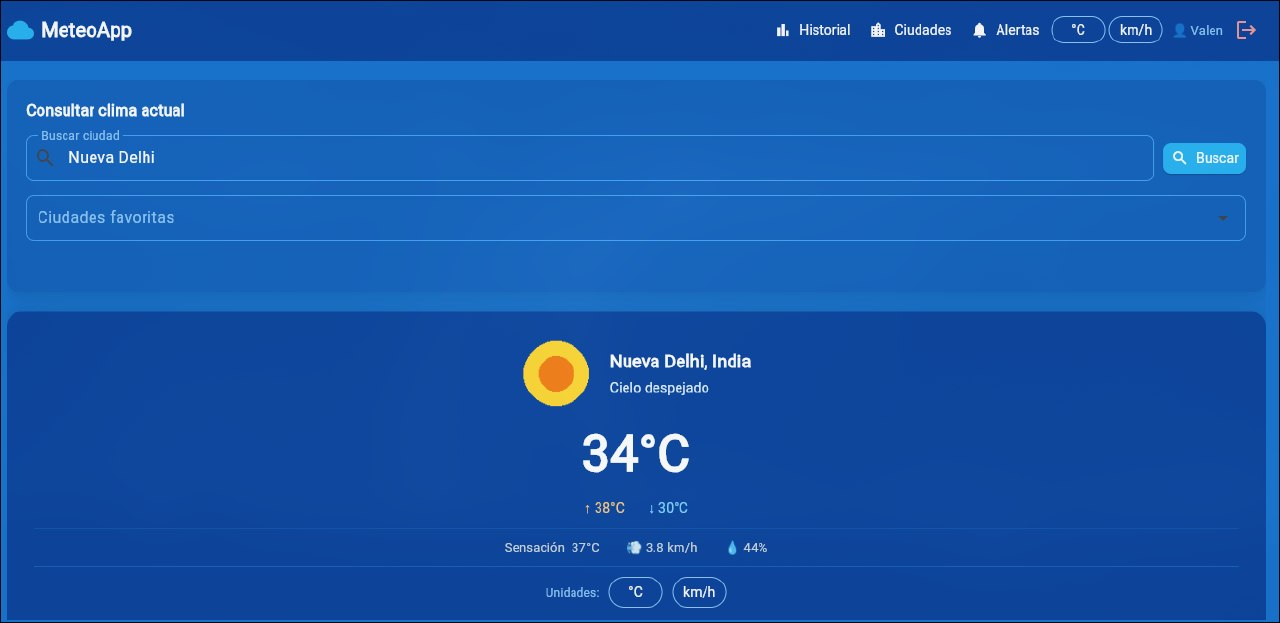
\includegraphics[width=0.85\textwidth]{assets/screenshots/home_weather.png}
    \caption{Pantalla principal mostrando el clima actual de una ciudad con tarjeta de datos.}
\end{figure}
\subsection{Cambio de unidades}
Los botones de unidad en la cabecera y en la tarjeta del clima permiten alternar entre:
\begin{itemize}
    \item °C / °F para temperatura.
    \item km/h / mph para velocidad del viento.
\end{itemize}
Las conversiones se aplican en tiempo real sin volver a consultar la API.
\subsection{Agregar ciudad a favoritas}
Al consultar una ciudad que no está en la lista de favoritas, aparece un diálogo preguntando si se desea agregarla. También se puede ir a la vista de Ciudades y agregar manualmente.
\begin{figure}[h]
    \centering
    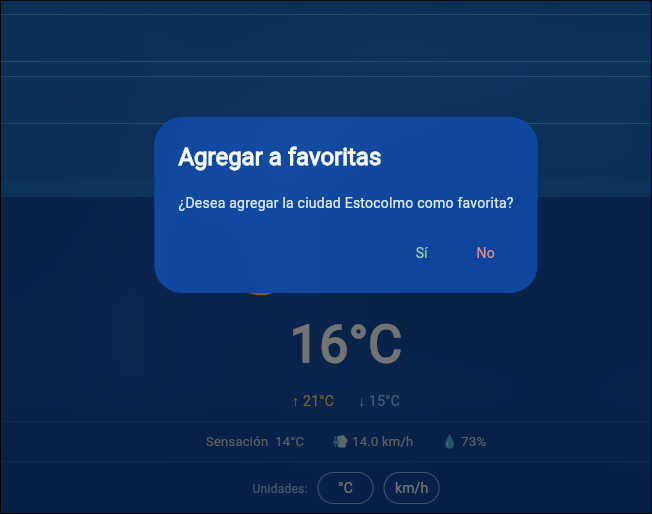
\includegraphics[width=0.6\textwidth]{assets/screenshots/favorite_dialog.png}
    \caption{Diálogo para agregar ciudad a favoritas.}
\end{figure}
\subsection{Gestión de ciudades favoritas}
Desde la vista "Ciudades" se puede:
\begin{itemize}
    \item Ver la lista de ciudades guardadas con su país.
    \item Agregar nuevas ciudades escribiendo el nombre.
    \item Eliminar ciudades seleccionándolas con checkboxes y haciendo clic en "Eliminar seleccionadas".
\end{itemize}
\begin{figure}[h]
    \centering
    \includegraphics[width=0.85\textwidth]{assets/screenshots/cities.png}
    \caption{Vista de gestión de ciudades favoritas con checkboxes.}
\end{figure}
\subsection{Historial meteorológico}
Desde la vista "Historial":
\begin{enumerate}
    \item Seleccionar una ciudad favorita del menú desplegable.
    \item Elegir una fecha de inicio con el selector de fecha.
    \item Ajustar la cantidad de días con el slider (7 a 183).
    \item Hacer clic en "Consultar historial".
\end{enumerate}
La aplicación genera dos gráficas:
\begin{itemize}
    \item \textbf{Temperatura:} gráfica de líneas con máxima (rojo) y mínima (azul).
    \item \textbf{Precipitación:} gráfica de barras con lluvia acumulada diaria en mm.
\end{itemize}
Además, se muestran estadísticas del período: promedio de temperatura máxima, mínima y lluvia.
\begin{figure}[h]
    \centering
    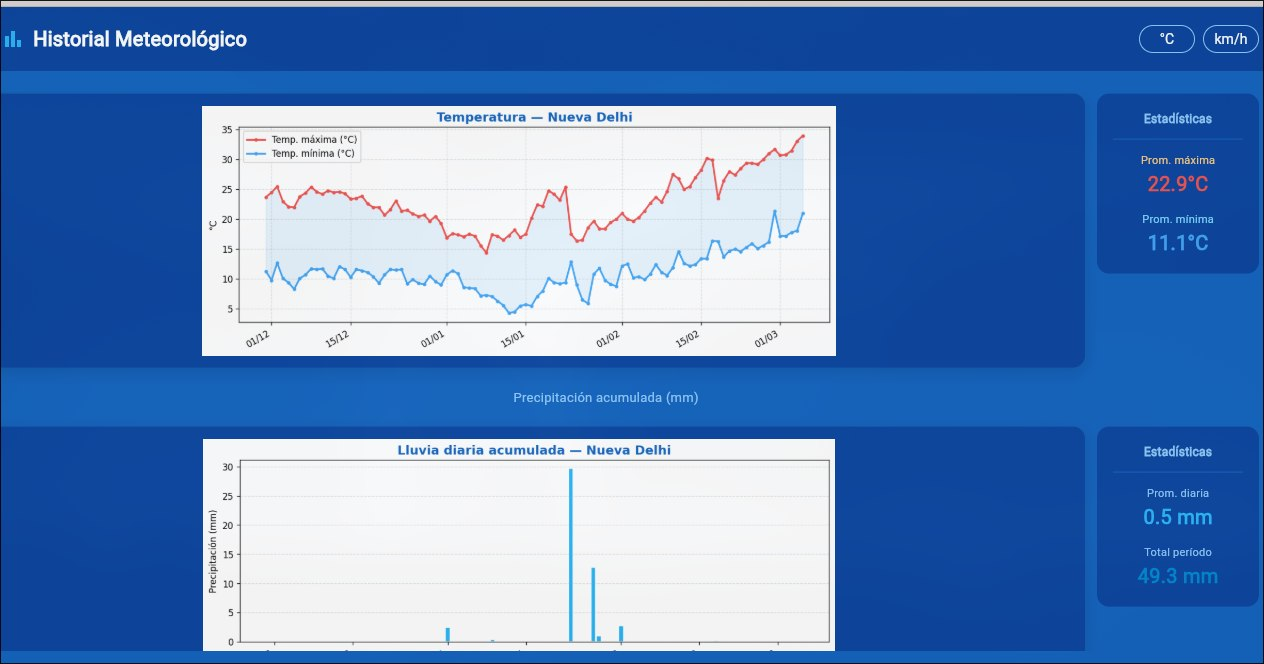
\includegraphics[width=0.85\textwidth]{assets/screenshots/history.png}
    \caption{Historial meteorológico con gráficas de temperatura y precipitación.}
\end{figure}
\subsection{Alertas de temperatura}
Desde la vista "Alertas":
\begin{enumerate}
    \item Seleccionar una ciudad favorita.
    \item Ajustar los umbrales de temperatura máxima y mínima con los sliders.
    \item Activar la alerta con el checkbox.
    \item Hacer clic en "Guardar configuración".
\end{enumerate}
Cuando la temperatura actual de una ciudad favorita supera el umbral configurado, aparece un banner rojo en la pantalla principal.
\begin{figure}[h]
    \centering
    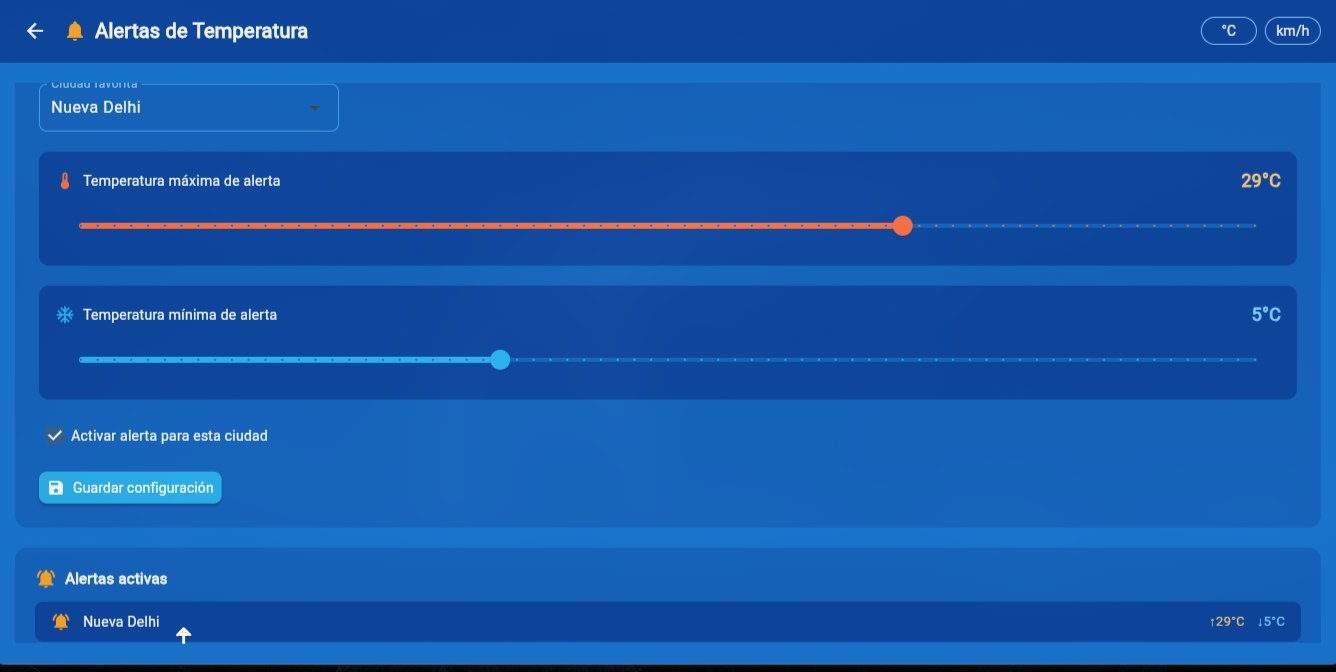
\includegraphics[width=0.85\textwidth]{assets/screenshots/alerts.png}
    \caption{Configuración de alertas de temperatura con sliders y resumen de alertas activas.}
\end{figure}
\subsection{Modo offline}
Si no hay conexión a internet al consultar una ciudad, la aplicación muestra automáticamente el último clima guardado en caché con un banner naranja indicando "Sin internet" y la fecha del último dato disponible.
\begin{figure}[h]
    \centering
    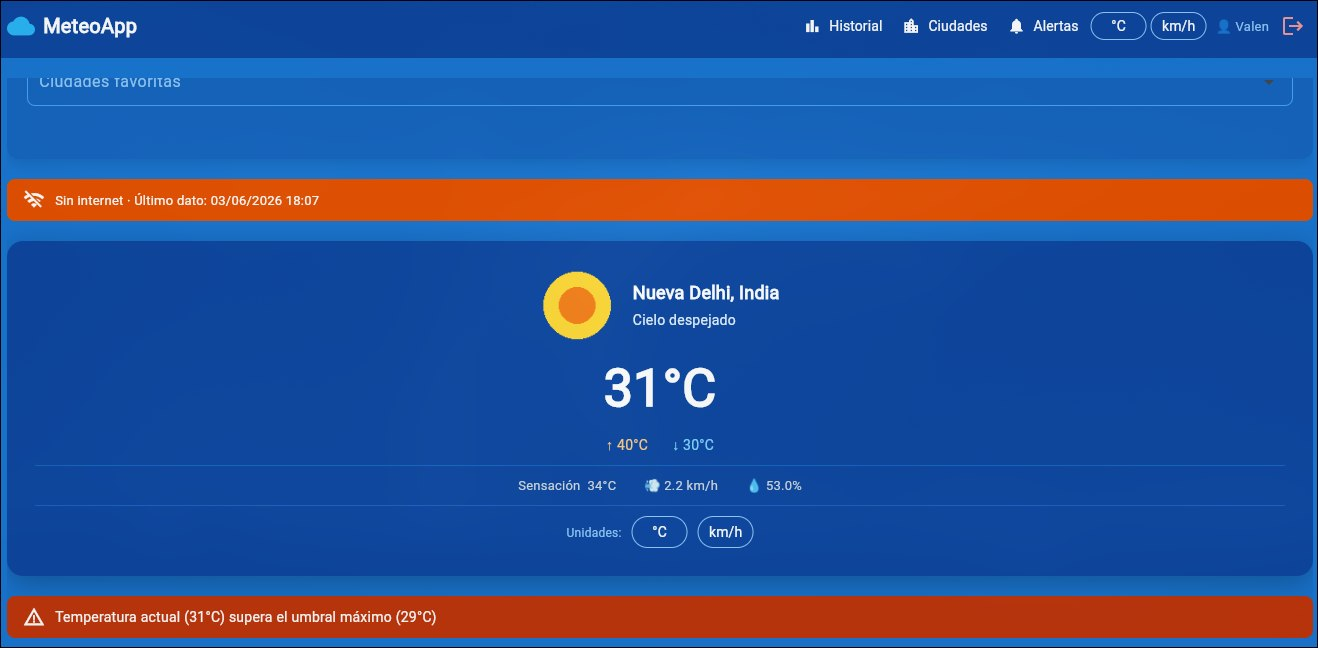
\includegraphics[width=0.85\textwidth]{assets/screenshots/offline.png}
    \caption{Modo offline: la aplicación muestra datos cacheados con aviso de conexión perdida.}
\end{figure}
\subsection{Ejemplo de gráficas generadas}
A continuación se muestran ejemplos de las gráficas que genera la aplicación con Matplotlib:
\begin{figure}[h]
    \centering
    \begin{minipage}{0.48\textwidth}
        \centering
        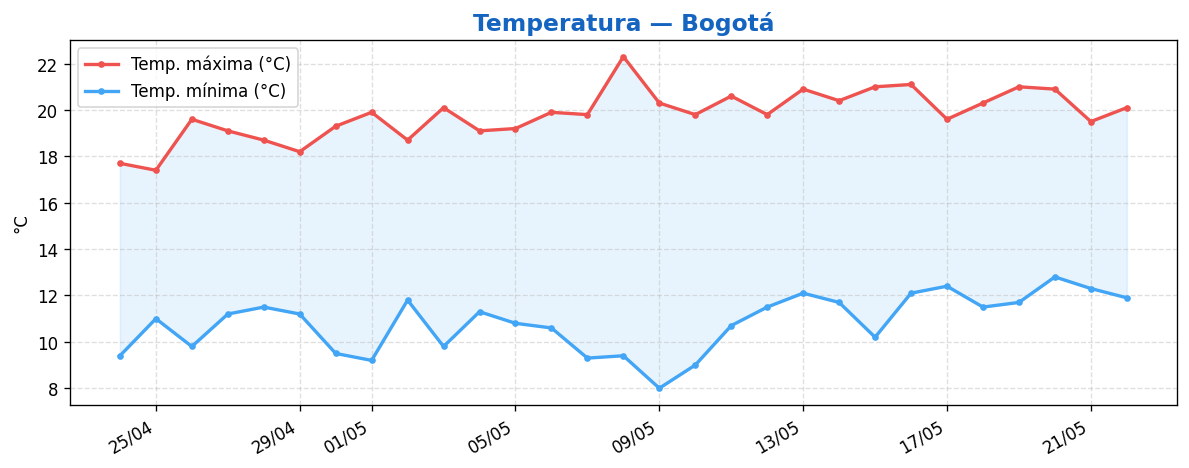
\includegraphics[width=\textwidth]{assets/charts/temperatura_bogotá.png}
        \caption{Gráfica de temperatura máxima y mínima.}
    \end{minipage}
    \hfill
    \begin{minipage}{0.48\textwidth}
        \centering
        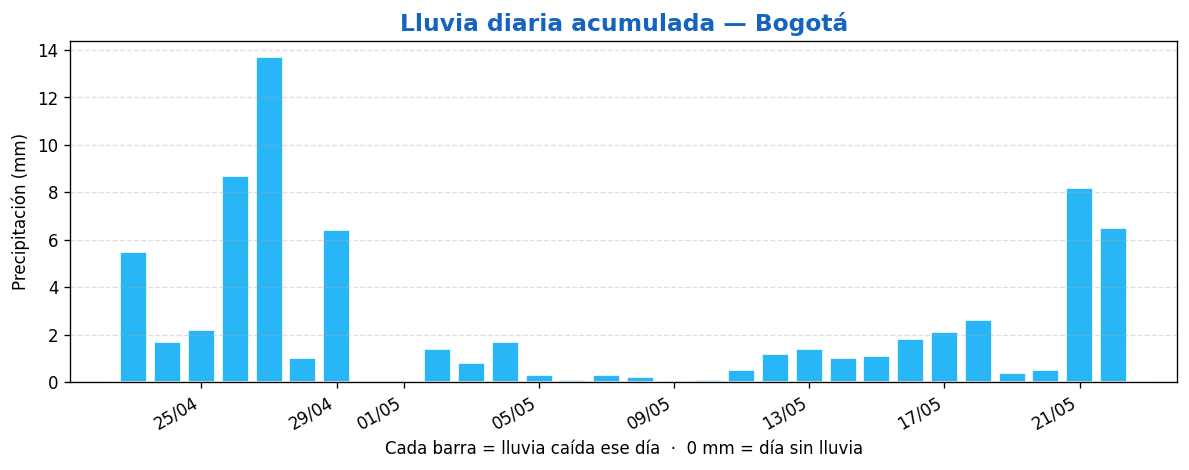
\includegraphics[width=\textwidth]{assets/charts/precipitacion_bogotá.png}
        \caption{Gráfica de precipitación acumulada.}
    \end{minipage}
\end{figure}
% ===============================================================================
\section{Pasos para Instalar y Ejecutar}
% ===============================================================================
\subsection{Requisitos}
\begin{itemize}
    \item Python 3.10 o superior (solo la primera vez para compilar; el ejecutable final no requiere Python instalado).
    \item Conexión a internet (para consultar la API; la aplicación también funciona offline con datos cacheados).
\end{itemize}

\subsection{Opción A: Ejecutable (Windows) -- Recomendado}

La forma más sencilla de usar la aplicación es mediante el ejecutable compilado. Solo se requiere hacer la compilación una vez:

\begin{enumerate}[itemsep=4pt]
    \item Abrir la carpeta del proyecto.
    \item Hacer doble clic en \texttt{build\_windows.bat} (solo la primera vez). Este script instala las dependencias y compila \texttt{MeteoApp.exe} automáticamente.
    \item Al finalizar, aparecerá \texttt{MeteoApp.exe} en la carpeta raíz del proyecto.
    \item Para ejecutar la aplicación, hacer doble clic en \texttt{MeteoApp.exe}.
\end{enumerate}

\noindent\textbf{Nota:} en futuras ocasiones no es necesario volver a ejecutar \texttt{build\_windows.bat}. Basta con hacer doble clic en \texttt{MeteoApp.exe}.

\subsection{Opción B: Desde el código fuente}

Si se desea ejecutar directamente con Python (por ejemplo, para modificar el código o para sistemas Linux/macOS):
\begin{lstlisting}[frame=none, numbers=none, basicstyle=\ttfamily\small]

# 1. Descargar y descomprimir el archivo .zip

# 2. Crear y activar entorno virtual

python3 -m venv .venv  (cambia el comando si está usando Anaconda en windows )
source .venv/bin/activate      # Linux/Mac
# .venv\Scripts\activate       # Windows

# 3. Instalar dependencias
python -m pip install --upgrade pip
pip install -r requirements.txt

# 4. Ejecutar la aplicacion
python main.py
\end{lstlisting}
% ===============================================================================
\section{Conclusiones y Posibles Mejoras}
% ===============================================================================
\subsection{Conclusiones}
El desarrollo de MeteoApp demostró que es posible construir una interfaz gráfica funcional y atractiva utilizando exclusivamente Python con la biblioteca Flet, integrando consumo de APIs externas, persistencia de datos en CSV y generación de gráficas en tiempo real. La arquitectura modular basada en POO permitió separar claramente la lógica de negocio (\texttt{utils/}) de la presentación (\texttt{views/}), facilitando el mantenimiento y la escalabilidad del código.
Se logró implementar un flujo completo de usuario: autenticación, consulta de clima actual con geocodificación, historial meteorológico con gráficas comparativas, gestión de ciudades favoritas y un sistema de alertas configurables. El manejo de errores de red y la caché offline aseguran que la aplicación degrade gracefully cuando no hay conexión a internet.
\subsection{Posibles mejoras}
\begin{itemize}
    \item \textbf{Internacionalización (i18n):} Agregar soporte para múltiples idiomas (inglés, portugués, etc.) usando un archivo de traducciones.
    \item \textbf{Base de datos SQLite:} Reemplazar los CSV por SQLite para consultas más rápidas y evitar problemas de concurrencia.
    \item \textbf{Notificaciones del sistema:} Enviar notificaciones nativas del sistema operativo cuando se active una alerta de temperatura, incluso si la app está minimizada.
    \item \textbf{Pronóstico extendido:} Mostrar el pronóstico de los próximos 7 días con tendencias climáticas.
    \item \textbf{Exportación de datos:} Permitir exportar el historial meteorológico a PDF o Excel.
    \item \textbf{Modo oscuro:} Agregar un tema oscuro configurable por el usuario.
    \item \textbf{Autenticación mejorada:} Implementar registro con confirmación de correo y recuperación de contraseña.
\end{itemize}
\vfill
\begin{center}
\rule{0.5\textwidth}{0.4pt}\\[0.3cm]
\textit{Manual de Usuario -- MeteoApp}\\[0.1cm]
\textit{Valentina Rodriguez Sepulveda -- 1125789977}\\[0.1cm]
\textit{2026}
\end{center}
\end{document}